\documentclass[11pt]{article}
\usepackage[margin=1in]{geometry}
\usepackage{amsmath}
\usepackage{amssymb}
\usepackage{graphicx}
\usepackage{booktabs}
\usepackage{hyperref}
\usepackage{authblk}
\usepackage{caption}

\hypersetup{
    colorlinks=true,
    linkcolor=blue,
    citecolor=blue,
    urlcolor=blue
}

\title{Hole Coverage and Rotational Symmetry Both Affect Fundamental Bending-Mode Frequency in Quasicrystal-Perforated MEMS Plates: A Finite-Element Study}
\author[1]{Gavin Branaa}
\affil[1]{Independent researcher}
\date{}

\begin{document}
\maketitle

\begin{center}
\textit{Draft --- prepared for preprint/submission. Computational study; no experimental fabrication or measurement was performed.}
\end{center}

\begin{abstract}
The question I had was whether symmetry order (3/6/8/12-fold) independently affects a quasicrystal-perforated MEMS plate's fundamental bending frequency, or whether hole coverage (density) dominates instead. To test this, I used a Mindlin-Reissner plate element --- this model is needed because, at this plate's thickness, you have to account for flex (shear), not just simple bending. Before trusting any results, I verified the model against the Leissa (1969) benchmark, because the mathematical baseline needed to be confirmed first.

Most of this work turned out to be finding and fixing my own mistakes, and three separate ones surfaced. My first method for representing holes --- deleting a mesh square whenever its center point fell inside a hole, all or nothing --- quietly broke the plate into disconnected islands, like stepping stones cut off from the mainland, and got \textit{worse}, not better, as I refined the mesh. I replaced it with a percentage-based method that scales each square by how much solid material it still has, so nothing ever creates a hard, disconnecting gap. Two more flaws surfaced the same way: a stiffness-weakening rule I had left as an arbitrary choice (later resolved by using a very fine mesh as a neutral answer key, which pointed to one specific rule), and a real bug in the code that generated the hole patterns themselves, which had been producing far sparser patterns than intended. The common thread is uncomfortable but worth stating plainly: each flaw produced results that looked perfectly reasonable, and each survived precisely because a result that matched what I already expected got less scrutiny than a contradicting one would have --- the hole-pattern bug, for instance, only surfaced when I sat down to write a precise description of the algorithm and the math stopped adding up.

With all three corrected, the answer is that hole coverage and symmetry order both affect the plate's fundamental frequency, but not equally. Coverage is the dominant knob; symmetry order is a real but secondary effect that is undetectable at near-dense coverage and switches on, growing steadily, as more material is removed. I also tested a second, separate quantity --- the bandgap, the empty frequency range between two vibration modes. My first, pre-correction attempt found no symmetry effect on it, and I wrote that up as a point of contrast with the photonic-quasicrystal literature, where symmetry is known to matter; after the corrections, a real trend appeared instead --- higher symmetry, wider gap --- which agrees with that literature rather than contradicting it. In that case the corrections did not just adjust a number, they reversed a conclusion.
\end{abstract}

\section{Introduction}

Quasicrystals --- structures with long-range order but no translational periodicity --- can exhibit rotational symmetries (5-, 8-, 12-fold, etc.) forbidden to conventional periodic crystals. This property has been exploited in photonic quasicrystals to produce large, highly isotropic complete photonic bandgaps unavailable to periodic structures of comparable complexity \cite{florescu2009}. More recently, the same design philosophy has been applied mechanically: Li, Cho, Norte \& Shin (2026) demonstrated a 12-fold quasicrystal-architected nanomechanical resonator achieving a mechanical quality factor $Q_m \approx 10^7$ and force sensitivity of 26.4~aN/$\sqrt{\text{Hz}}$, via a data-driven hole-pattern optimization that exploits aperiodic order to relax the symmetry constraints limiting periodic phononic-crystal ``soft clamping'' designs \cite{li2026}.

A practical question follows directly from this line of work: when designing a quasicrystal-perforated resonator, is the rotational symmetry order itself a meaningful, independent tuning parameter for the device's fundamental frequency --- or does frequency depend primarily on the more easily controlled parameter of how much material is removed (hole coverage)? Coverage is trivial to control during fabrication (hole size, spacing density); achieving a specific high-fold rotational symmetry is a more demanding geometric and fabrication constraint. The practical value of an answer depends on its direction: if symmetry order is irrelevant, designers can use simpler, lower-fold patterns without performance cost; if it has a real, independent effect, it is a genuine design parameter worth the added fabrication complexity, at least in some coverage regimes.

This question is distinct from the analogous, well-studied question in 2D photonic quasicrystals, where symmetry order is known to affect \textbf{complete bandgap width}: Florescu, Torquato \& Steinhardt (2009) report optimized complete photonic bandgaps of 16.5\% (5-fold) and 13.5\% (8-fold) for comparable optimized structures \cite{florescu2009}. That result concerns bandgap \textit{width}, a different quantity from the single fundamental-mode \textit{frequency} tested in the present mechanical study, and the two should not be conflated.

We address the mechanical question with a finite-element model of a clamped, quasicrystal-perforated silicon plate. A substantial part of this study, reported in Section~\ref{sec:methods-element}, concerns a methodological correction made partway through: an initial hole-geometry implementation was found to be unreliable across the full range tested, not just at low coverage as first suspected, and was replaced with a more robust formulation before the results reported in Section~\ref{sec:results} were finalized.

\section{Methods}

\subsection{Material and geometry}

A $100\times100\,\mu$m square silicon plate ($E = 170$~GPa, $\nu = 0.28$, $\rho = 2330$~kg/m$^3$, thickness $h = 100$~nm), fully clamped on all four edges (CCCC boundary condition), perforated with a quasiperiodic hole pattern generated via the de Bruijn multigrid construction (the algorithm underlying Penrose and Ammann-Beenker tilings, generalized here to arbitrary $n$-fold rotational symmetry).

\textbf{Construction details.} $n_{\text{fold}}$ families of parallel lines are placed, one family per direction $\theta_k = k\pi/n_{\text{fold}}$ ($k = 0,\ldots,n_{\text{fold}}-1$); within family $k$, lines are spaced one unit apart along that family's perpendicular and offset by an independent random phase $\gamma_k$ drawn uniformly from $[0,1)$. Hole centers are placed at every pairwise intersection of a line from one family with a line from a different family --- line $m$ of family $k$ is the set of points $P$ satisfying $P\cdot\hat{n}_k = m + \gamma_k$, where $\hat{n}_k$ is the unit normal to direction $k$. Each candidate intersection is computed by solving the corresponding $2\times2$ linear system exactly. The resulting point pattern is scaled to fit the $100\times100\,\mu$m domain (scale factor $0.45\times$ the domain's shorter side) and re-centered; points falling outside the domain after scaling are discarded, and near-duplicate points (closer than 5\% of the scale factor --- a degeneracy that can occur where more than two line families happen to intersect very near the same location) are removed, keeping the first-found point of each cluster.

\textbf{A methodological correction worth recording.} An earlier version of this construction contained a real implementation bug: although both line indices ($m$ for family $i$, $m'$ for family $j$) were looped over when generating candidate intersections, the position formula in that version only used $m$, never $m'$ --- meaning every candidate intersection for a given line-pair-and-$m$ actually returned the same point regardless of $m'$, collapsing what should have been a full 2D grid of pairwise intersections (typically tens to hundreds of points per direction-pair within the domain) down to a single line's worth of points (one per $m$, $\sim$17 points) per direction pair. We discovered this only when attempting to write a precise description of the construction for this section, by directly checking whether varying the unused index actually changed the computed point --- it did not. This explains several previously-documented, but previously-unexplained, oddities throughout this study's earlier results: persistently low candidate-point counts at low symmetry order ($n=3$ had only $\sim$5 candidate points under the old construction, vs.\ 12 under the fix), an inability to coverage-match $n=3$ to 80\% even at large search radii (resolved entirely under the fix --- see Section~\ref{sec:symmetry-protocol}), and elevated, $n=3$-specific seed-to-seed noise attributed throughout earlier sections of this study to ``low candidate-point count'' --- a real phenomenon, but one substantially caused by this implementation bug rather than being an unavoidable property of low-fold de Bruijn constructions. The fix was verified two ways: (1) directly, by confirming each solved intersection point satisfies both line equations to floating-point precision, and (2) by checking that resulting point counts scale sensibly with symmetry order (12, 39, 79, and 140 points for $n=3$, 6, 8, and 12 respectively, at the parameters used throughout this study) and saturate as the line-index search range is widened, confirming all in-domain intersections are captured. All results reported in this manuscript use the corrected construction, including the coverage sweep (Section~\ref{sec:results}) and the uncontrolled symmetry sweep (Section~\ref{sec:confound}), both subsequently re-run with it (Section~\ref{sec:limitations}).

\subsection{Finite element formulation}
\label{sec:methods-element}

Plate bending was modeled with a 4-node bilinear Mindlin-Reissner plate element. Each node carries 3 degrees of freedom: transverse deflection $w$ and two independent rotation fields $\theta_x, \theta_y$.

\textbf{Element formulation.} Standard bilinear isoparametric shape functions $N_{1-4}(\xi,\eta)$ on the reference square $[-1,1]^2$, with physical-coordinate derivatives via the isoparametric Jacobian. Bending curvatures are obtained from the rotation fields ($\kappa_{xx} = \partial\theta_x/\partial x$, $\kappa_{yy} = \partial\theta_y/\partial y$, $2\kappa_{xy} = \partial\theta_x/\partial y + \partial\theta_y/\partial x$); bending stiffness $K_b$ uses the constitutive matrix
\[
D_b = D \begin{bmatrix} 1 & \nu & 0 \\ \nu & 1 & 0 \\ 0 & 0 & (1-\nu)/2 \end{bmatrix}, \quad D = \frac{Eh^3}{12(1-\nu^2)},
\]
with full $2\times2$ Gauss quadrature. Shear strains ($\gamma_{xz} = \partial w/\partial x - \theta_x$, $\gamma_{yz} = \partial w/\partial y - \theta_y$) use the physical, unfitted shear stiffness $G_s = \kappa G h$ ($\kappa=5/6$, $G=E/[2(1+\nu)]$) with Selective Reduced Integration (1-point centroid quadrature for shear, full quadrature for bending and mass) --- the standard SRI locking remedy \cite{hughes1978,hughes1981} for this MEMS-scale thickness ratio ($h/L \approx 1\times10^{-3}$). An earlier 3-node triangular element using a mesh-fitted (non-physical) shear stiffness was discarded after deviating from the analytical benchmark below by 36\%.

\textbf{Hole representation --- an initial approach found to be flawed, and its replacement.} Holes were initially represented by binary element removal: an element was voided from the mesh entirely if its centroid fell within a hole's radius. This is a common, simple approach, but over the course of this study (Section~\ref{sec:earlier-phase} describes the original results obtained with this method, for context) it was found to produce a serious, previously undiagnosed problem: the resulting mesh geometry fragments into many disconnected components, with the fragment count \textit{growing} under mesh refinement rather than converging to a fixed value, at every coverage level eventually tested --- including the originally-tested $\sim$98\% coverage configuration, where the effect was small enough (single-digit fragment counts at the coarse mesh resolutions first used) to go undetected. This rules out simple under-resolution as the cause; it reflects the binary removal scheme's sensitivity to how overlapping circular holes intersect at the sub-element scale, which a single-point (centroid) inclusion test cannot represent faithfully at any finite resolution. A 90\%-coverage spot-check, performed specifically to see whether the problem extended beyond 98\% coverage, initially appeared fragmentation-free --- but this was later found to be an error in the check itself, not a property of 90\% coverage: the verification had been run against the \textit{98\%-coverage} hole radii by mistake, not the 90\%-coverage radii it was meant to test. Once corrected to use the actual 90\%-coverage radii, the same unbounded fragmentation problem appeared there as well (Section~\ref{sec:limitations-discussion} discusses this as a specific instance of a broader pattern in this study).

\textbf{Corrected method: area-fraction homogenization.} Each element's stiffness and mass matrices are scaled by $\phi \in [0,1]$, the fraction of the element's physical area \textit{not} covered by any hole, computed by regular sub-sampling ($12\times12$ sample points per element) rather than a single centroid test:
\[
K_e = \phi \cdot (K_b + K_s), \qquad M_e = \phi \cdot M_{e,\text{full}}
\]
with $\phi$ floored at $10^{-3}$ (rather than allowed to reach exactly 0) to avoid a singular mass matrix for elements entirely inside a hole --- a standard regularization in SIMP-style topology-optimization penalization, contributing negligible stiffness/mass while keeping the eigenproblem well-posed. We tested whether this specific floor value matters: holding hole geometry fixed ($n=8$, $\sim$80\% coverage) and varying the floor across three orders of magnitude ($10^{-2}$, $10^{-3}$, $10^{-4}$, $10^{-5}$), $f_1$ changed by no more than 0.39\% relative to the chosen value ($10^{-3}$), and the result had already converged by $10^{-4}$ ($10^{-4}$ and $10^{-5}$ agree to within 0.001\%) --- confirming $10^{-3}$ sits safely in the regularization's insensitive regime rather than being an arbitrary, untested choice. This is a homogenization approximation, not an exact sub-element-scale geometric representation (which would require true conformal/constrained-Delaunay meshing of the hole boundaries); it is, however, structurally immune to the disconnection failure mode of binary removal, since no element's properties are ever discontinuously zeroed except in the (regularized) limit of complete coverage. All results reported in Section~\ref{sec:results} use this corrected method.

\subsection{Verification against an analytical benchmark}

Both the binary-removal and homogenized methods reduce to the same unperforated-plate problem when no holes are present, and were verified identically against the Leissa (1969) analytical solution for a clamped square plate (CCCC) \cite{leissa1969}:

\begin{table}[h]
\centering
\caption{Convergence to the Leissa clamped-plate benchmark.}
\begin{tabular}{cccc}
\toprule
Mesh ($n_x$) & Nodes & FEM $f_1$ (MHz) & FEM/Analytical \\
\midrule
10 & 100 & 0.1520 & 1.033 \\
16 & 256 & 0.1488 & 1.012 \\
22 & 484 & 0.1480 & 1.006 \\
30 & 900 & 0.1476 & 1.003 \\
\bottomrule
\end{tabular}
\end{table}

Analytical $f_1 = 0.1471$~MHz. Convergence is monotonic and clean, with no evidence of shear locking (Figure~\ref{fig:convergence}). Independently reproduced on a separate machine (no access to original code/output): identical ratios at all four resolutions.

\begin{figure}[h]
\centering
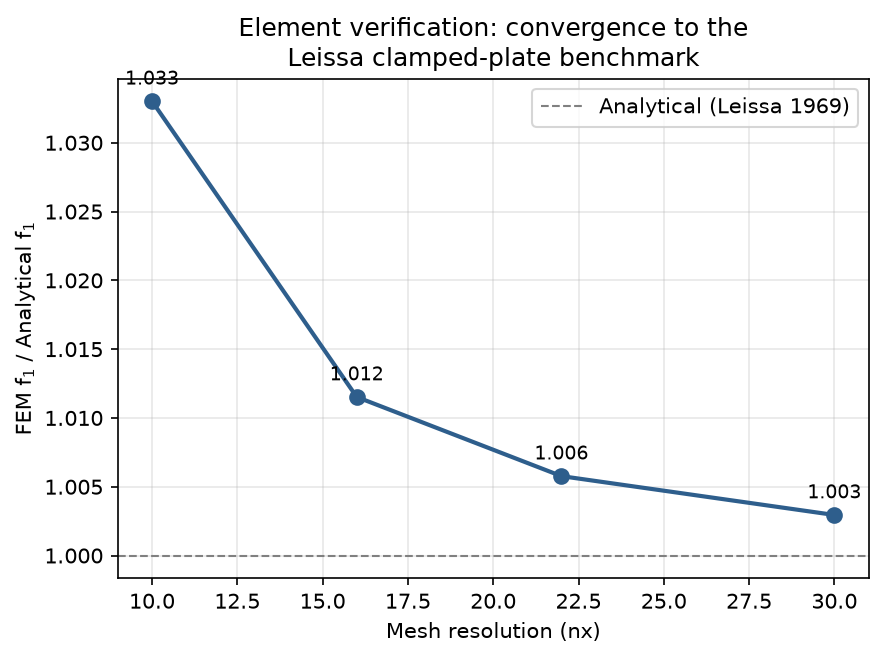
\includegraphics[width=0.7\textwidth]{figure_convergence.png}
\caption{FEM/analytical frequency ratio vs. mesh resolution for the clamped-plate benchmark.}
\label{fig:convergence}
\end{figure}

With holes present, the homogenized method was further verified to converge smoothly under mesh refinement (no fragmentation artifact) at the most demanding configuration tested ($n=8$, $r=3.5\,\mu$m, $\sim$89\% coverage): $f_1 = 0.1468 / 0.1451 / 0.1440 / 0.1431 / 0.1427$~MHz at $n_x = 22/32/44/60/80$ --- a smooth, monotonically converging sequence, in contrast to the binary-removal method's component count at the same configuration ($6/79/213/440$ at $n_x = 22/44/60/80$), which grew without bound.

\subsection{Coverage sweep}

Hole radius was swept at fixed symmetry order ($n=8$) and fixed mesh ($22\times22$), with coverage computed as the mean element area fraction $\phi$. This sweep used the default (linear, $\phi^1$) stiffness scaling, predating the exponent resolution in Section~\ref{sec:exponent}; see the caveat in Section~\ref{sec:results} (Coverage controls fundamental frequency) regarding comparability with the later, quadratic-exponent results. Re-run with the corrected de Bruijn geometry (Section~\ref{sec:methods-element}) at the same fixed radii (Section~\ref{sec:results}).

\subsection{Symmetry sweep, uncontrolled}

Symmetry order was swept ($n = 3, 6, 8, 12$) at a nominally fixed hole radius, uncovering a coverage confound described in Section~\ref{sec:confound}. Re-run with the corrected de Bruijn geometry (Section~\ref{sec:methods-element}) at a fixed radius (2.5~$\mu$m), $n_x=28$, 3 seeds per symmetry order.

\subsection{Symmetry sweep, coverage-matched, at three coverage levels}
\label{sec:symmetry-protocol}

For each symmetry order, hole radius was tuned via per-configuration bisection search (mesh $n_x=28$) to match target coverage (98\%, 90\%, and 80\%, each $\pm0.4\%$), removing coverage as a confounding variable. Five independent de Bruijn tiling phase-offset realizations (seeds) were tested per symmetry order at each coverage level for the final (quadratic-exponent, Section~\ref{sec:exponent}) results; an earlier pass with an unresolved (linear) exponent choice and the pre-fix geometry is summarized for comparison in Section~\ref{sec:earlier-phase}. Mesh convergence ($n_x = 24, 28, 34$) was measured directly on one representative configuration ($n=8$) at each coverage level, providing a noise floor specific to each comparison.

\subsection{Independent cross-validation against the corrected methodology}
\label{sec:crossval}

A second, independently-coded element was used to cross-check the corrected (homogenized, quadratic-exponent) results in Section~\ref{sec:results}. The first candidate for this role, a 3-node linear Mindlin triangle (different shape functions and mesh topology from the paper's main 4-node quad element, originally reported against the now-superseded binary-removal results), was re-tested directly against the analytical Leissa benchmark and found unsuitable: it is locked by 19.7$\times$ at a coarse mesh and still 2.5$\times$ at 14{,}400 nodes --- roughly nine times the node count of the working quad mesh --- never converging in any practical regime at this plate's thickness ratio ($h/L_x \approx 1\times10^{-3}$), because its constant (single-point) shear strain field has no relief mechanism. This element was discarded for cross-validation purposes.

It was replaced with a 6-node quadratic Mindlin triangle (LST topology: 3 corner + 3 generated mid-edge nodes, on a Delaunay-triangulated mesh --- still a fundamentally different element family and mesh-generation path from the quad), homogenized with the same area-fraction, quadratic-exponent approach as the main results. A first attempt copied the quad element's selective-reduced-integration (SRI) strategy literally (single-centroid-point shear integration) and produced a rank-deficient stiffness matrix (negative/near-zero eigenvalues, i.e., spurious zero-energy ``hourglass'' modes) --- this element's shear field is naturally degree-2 (same order as bending), so a single integration point under-constrains it, unlike the bilinear quad's degree-1 shear field, for which 1-point reduction is the textbook-correct SRI choice. Using the same 3-point Gauss rule for both bending and shear (full, consistent integration, not SRI) resolved this and converged cleanly against the Leissa benchmark (ratio 1.28 at a coarse mesh, 1.02 at 2{,}209 nodes) --- comparable convergence quality to the main quad element.

Using this validated element and the corrected de Bruijn geometry (Section~\ref{sec:methods-element}), coverage-matched (80\% target) radii were re-derived independently per seed (not copied from the quad element's results), and the symmetry comparison was re-run with 5 seeds per symmetry order, all four symmetry orders included (the $n=3$ coverage-matching ceiling present under the earlier, buggy geometry construction does not recur under the corrected one --- Section~\ref{sec:limitations}). The cross-validation element found a 3.50\% spread across all four symmetry orders ($n=3$: 0.1433~MHz, $n=6$: 0.1404~MHz, $n=8$: 0.1406~MHz, $n=12$: 0.1384~MHz) --- a real, modest, nonzero effect, qualitatively corroborating Section~\ref{sec:results}'s finding of a real symmetry-order effect at sub-90\% coverage. The exact magnitude differs from the quad element's 80\%-coverage spread (4.86\%, Section~\ref{sec:results}); this is expected and was never the standard for this comparison --- independently-coded elements with different shape functions, integration order, and mesh topology are not expected to reproduce identical absolute numbers, only the qualitative conclusion, which they do.

\section{Results}
\label{sec:results}

\textbf{Summary of findings (author's own words):} Reducing hole coverage from 98\% to 80\% reduced the plate's frequency by 10.51\% --- less material means less stiffness, so the frequency drops as more is removed. The symmetry-order effect was smaller and depended on coverage: undetectable at 98\% coverage (0.15\% spread vs.\ 0.26\% expected noise), but clearly real by 90\% (1.22\% vs.\ 0.61\% noise) and even more clearly by 80\% (4.86\% vs.\ 0.89\% noise). I resolved the earlier uncertainty about how strongly a partially-covered square should lose stiffness by using a finer mesh grid as a calibration check --- checking which of two competing weakening rules was actually closer to correct --- and the numbers above reflect the answer that calibration gave. The full data and technical detail behind this summary follow below.

\subsection{Coverage controls fundamental frequency}

Re-run with the corrected de Bruijn geometry (Section~\ref{sec:methods-element}); pre-fix values, computed at the same fixed radii, are shown for comparison.

\begin{table}[h]
\centering
\caption{Density sweep, $n=8$, $n_x=22$, corrected geometry vs.\ pre-fix.}
\begin{tabular}{ccccc}
\toprule
Hole radius ($\mu$m) & Coverage (\%), corr. & $f_1$ (MHz), corr. & Coverage (\%), pre-fix & $f_1$ (MHz), pre-fix \\
\midrule
0.5 & 99.4 & 0.1480 & 99.8 & 0.1480 \\
1.5 & 94.7 & 0.1475 & 97.8 & 0.1480 \\
2.5 & 86.5 & 0.1453 & 94.1 & 0.1478 \\
3.5 & 77.2 & 0.1403 & 89.1 & 0.1468 \\
\bottomrule
\end{tabular}
\end{table}

A monotonic frequency reduction with decreasing coverage, confirmed smoothly convergent under mesh refinement at the most demanding (lowest-coverage) point tested. The effect size at this $n_x=22$ resolution and coverage range (99.4\%$\to$77.2\%) is $\sim$5.2\%, larger than the pre-fix sweep's $\sim$0.8\% over a narrower coverage range (99.8\%$\to$89.1\%) --- the corrected, denser hole pattern removes more material at the same radius (79 candidate points at this radius vs.\ far fewer pre-fix), reaching a wider, lower-coverage range at the same four radii tested. This is still not directly comparable to the 10.51\% coverage effect reported in Section~\ref{sec:symmetry-results}, which uses a different mesh resolution ($n_x=28$), a different, wider coverage range (98\%$\to$80\%), and the quadratic stiffness exponent resolved in Section~\ref{sec:exponent} (this sweep retains the linear exponent it was originally run with, for direct before/after comparability with the pre-fix values above); readers comparing effect sizes across sections should note these differences in conditions.

\subsection{An apparent symmetry effect, and a coverage confound}
\label{sec:confound}

Re-run with the corrected de Bruijn geometry (Section~\ref{sec:methods-element}): an uncontrolled symmetry sweep at a fixed hole radius (2.5~$\mu$m, $n_x=28$, linear exponent, 3 seeds per symmetry order) showed a spread of 5.91\% that on its own would suggest a substantial symmetry-order effect; closer examination found hole coverage was not in fact held constant across symmetry order (correlation between frequency and coverage, $r=0.96$, across this 12-run dataset) because the de Bruijn construction's candidate-point count scales strongly with symmetry order at fixed radius (12, 39, 79, and 140 points for $n=3$, 6, 8, and 12 respectively --- Section~\ref{sec:methods-element}), so coverage drops sharply with increasing $n_{\text{fold}}$ even though the hole radius itself never changes. This finding --- that an apparent symmetry effect can be substantially a coverage effect in disguise --- motivated the coverage-matched protocol used for all results below. (An earlier version of this sweep, using the pre-fix geometry, found a smaller spread of 1.44\% and correlation $r=0.92$ --- the same qualitative conclusion, with the corrected geometry's much stronger point-count-vs-symmetry-order scaling producing a larger, even more clearly confounded result.)

\subsection{Resolving the stiffness-penalization exponent}
\label{sec:exponent}

The homogenization (Section~\ref{sec:methods-element}) scales each element's stiffness by $\phi$, the surviving area fraction. The exponent on this scaling (linear, $\phi^1$, vs.\ quadratic, $\phi^2$, or other values) is a free modeling choice not fixed by the area-fraction calculation itself, and an initial sensitivity check found the symmetry-comparison results below were not robust to it. We resolved this directly: at sufficiently fine mesh resolution, individual elements no longer straddle hole boundaries (each element is either essentially fully covered or fully uncovered), so $\phi$ approaches 0 or 1 for every element and the exponent choice becomes irrelevant --- this gives an exponent-independent reference value to check coarser, computationally affordable meshes against. For a representative configuration ($n=8$, 80\% coverage target), linear and quadratic exponents converge toward the same value as mesh resolution increases ($f_1$ difference between the two: 7.03\% at $n_x=28$, shrinking to 1.51\% at $n_x=160$), confirming this approach is valid. At the working resolution used throughout this study ($n_x=28$), the quadratic exponent is closer to this fine-mesh reference value (linear overestimates by $\sim$5.9\%, quadratic underestimates by only $\sim$1.3\%) --- \textbf{the quadratic exponent is therefore the better-justified choice at this resolution, and all results below use it.} (This recheck used the corrected de Bruijn geometry described in Section~\ref{sec:methods-element}; the conclusion is unchanged from the original, pre-correction check.)

This single-configuration check ($n=8$, 80\% coverage) does not by itself establish that quadratic generalizes to other symmetry orders or coverage levels, so we repeated it at three additional configurations ($n=3$ and $n=12$ at 80\% coverage; $n=3$ and $n=8$ at 90\% coverage), comparing each exponent's $n_x=28$ result against a finer-mesh ($n_x=100$) reference. \textbf{Quadratic was closer to the reference in all four additional configurations tested} --- $n=3$/80\%: linear $+13.33\%$, quadratic $+10.77\%$; $n=12$/80\%: linear $+11.38\%$, quadratic $+0.57\%$; $n=8$/90\%: linear $+4.74\%$, quadratic $-0.22\%$; $n=3$/90\%: linear $+24.26\%$, quadratic $+21.49\%$ --- confirming the exponent choice generalizes beyond the single configuration originally checked, though quadratic's advantage is far more pronounced at $n=8$ and $n=12$ than at $n=3$. This comparison also surfaced a separate, previously-undisclosed finding: $n=3$ configurations show substantially larger mesh-resolution error at the working resolution (10--24\%, regardless of exponent) than $n=8$ or $n=12$ (0.2--11\%), meaning $n_x=28$ results for $n=3$ specifically should be treated as less numerically converged in an absolute sense than the other symmetry orders, independent of and in addition to $n=3$'s separately-documented seed-to-seed noise issues (Section~\ref{sec:limitations}). This does not invalidate the $n=3$ comparisons in Section~\ref{sec:symmetry-results} (the same systematic mesh-resolution bias affects all of $n=3$'s seeds in the same direction, so relative comparisons across seeds at fixed $n=3$ remain meaningful), but it is a real caveat on the absolute accuracy of $n=3$'s reported frequencies specifically.

\subsection{Coverage-matched symmetry comparison at three coverage levels (corrected methodology, quadratic exponent, corrected geometry)}
\label{sec:symmetry-results}

\begin{table}[h]
\centering
\caption{Symmetry-order spread vs. coverage, corrected methodology, quadratic exponent, corrected de Bruijn geometry.}
\begin{tabular}{cccc}
\toprule
Coverage & Across-$n_{\text{fold}}$ spread & Noise floor ($n=8$) & Spread/noise ratio \\
\midrule
98\% & 0.15\% & 0.26\% & spread $<$ noise --- \textbf{no detectable effect} \\
90\% & 1.22\% & 0.61\% & $\sim$2.0$\times$ --- \textbf{real effect} \\
80\% & 4.86\% & 0.89\% & $\sim$5.5$\times$ --- \textbf{real, clearly detectable effect} \\
\bottomrule
\end{tabular}
\end{table}

\begin{table}[h]
\centering
\caption{Per-symmetry-order means, with seed-to-seed standard deviation (5 seeds each, individually coverage-matched).}
\begin{tabular}{cccc}
\toprule
$n$-fold & $f_1$ (MHz), 98\% & $f_1$ (MHz), 90\% & $f_1$ (MHz), 80\% \\
\midrule
3 & 0.14598 ($\pm$0.44\%) & 0.14082 ($\pm$0.87\%) & 0.13601 ($\pm$1.19\%) \\
6 & 0.14613 ($\pm$0.28\%) & 0.13999 ($\pm$1.09\%) & 0.13168 ($\pm$2.16\%) \\
8 & 0.14620 ($\pm$0.15\%) & 0.13955 ($\pm$0.75\%) & 0.13083 ($\pm$0.48\%) \\
12 & 0.14610 ($\pm$0.17\%) & 0.13912 ($\pm$0.80\%) & 0.12959 ($\pm$1.92\%) \\
\bottomrule
\end{tabular}
\end{table}

These per-cell standard deviations capture seed-to-seed (geometric realization) variability and are a different quantity from the mesh-convergence noise floor reported above the table --- both matter, but for different reasons: the mesh-convergence noise floor tells us whether a given mean is numerically trustworthy at this mesh resolution, while the seed-to-seed standard deviation tells us how much any single realization's frequency can differ from its symmetry order's mean. Notably, the previously-assumed ``$n=3$ is the noisiest symmetry order'' pattern does not hold uniformly here --- at 80\% coverage, $n=6$ ($\pm$2.16\%) is noisier than $n=3$ ($\pm$1.19\%), a reversal from the pre-de-Bruijn-fix data and a reminder that this noise pattern is itself geometry-construction-dependent rather than a fixed property of any one symmetry order.

\textbf{Intermediate coverage levels.} The three coverage levels above (98\%, 90\%, 80\%) leave the functional form of the symmetry effect's growth uncharacterized between them. We tested two intermediate levels (94\%, 85\%; quadratic exponent, 3 seeds per symmetry order) to fill this gap:

\begin{table}[h]
\centering
\caption{Symmetry-order spread vs.\ coverage, including intermediate levels.}
\begin{tabular}{cccc}
\toprule
Coverage & Across-$n_{\text{fold}}$ spread & Noise floor ($n=8$) & Spread/noise ratio \\
\midrule
98\% & 0.15\% & 0.26\% & $<$1$\times$ --- no detectable effect \\
94\% & 0.85\% & 0.45\% & $\sim$1.9$\times$ --- real effect \\
90\% & 1.22\% & 0.61\% & $\sim$2.0$\times$ --- real effect \\
85\% & 3.95\% & 0.99\% & $\sim$4.0$\times$ --- real, clearly detectable effect \\
80\% & 4.86\% & 0.89\% & $\sim$5.5$\times$ --- real, clearly detectable effect \\
\bottomrule
\end{tabular}
\end{table}

Across all five coverage levels now tested, the spread grows smoothly and monotonically as coverage decreases, with no discontinuities or reversals --- the largest single jump occurs between 90\% and 85\% coverage (spread roughly tripling, from 1.22\% to 3.95\%), with comparatively smaller jumps elsewhere. Five points is still not enough to fit a specific functional form (e.g., linear vs.\ power-law in coverage loss) with confidence, but the smooth monotonic trend across five independently-tested points is itself a stronger confirmation of ``a real, growing effect'' than the original three-point table alone provided, and rules out any obvious non-monotonic behavior in this coverage range.

\textit{Coverage-matching note:} each of the 5 seeds was individually bisected to its own target-coverage radius (not a single shared radius reused across seeds), since the corrected, properly-dense de Bruijn geometry (Section~\ref{sec:methods-element}) varies enough seed-to-seed that a shared radius misses the target for individual seeds. All entries above are individually matched within $\pm0.4\%$ of the stated target. No outlier seeds were excluded from any of the means in this table --- the $n=3$, 80\%-coverage outlier present under the previous (buggy-geometry) construction does not recur under the corrected one (Section~\ref{sec:limitations}).

This is a cleaner result than the initial linear-exponent analysis suggested: \textbf{no detectable symmetry-order effect at near-dense (98\%) coverage, with a real effect emerging and growing as coverage decreases} --- clearly resolved from noise by 90\% coverage, and even more clearly by 80\%. The coverage effect over the same 98\%$\to$80\% range, computed from this table's $n=8$ column, is $(0.14620 - 0.13083)/0.14620 = \textbf{10.51\%}$ --- larger than the symmetry-order spread at every coverage level tested, consistent with coverage being the dominant variable, while symmetry order is a real, secondary, coverage-dependent effect rather than the negligible one our earlier, flawed (binary-removal) analysis had suggested.

Figure~\ref{fig:modeshapes} shows the first six mode shapes for a representative configuration ($n=8$, $\sim$98\% coverage).

\begin{figure}[h]
\centering
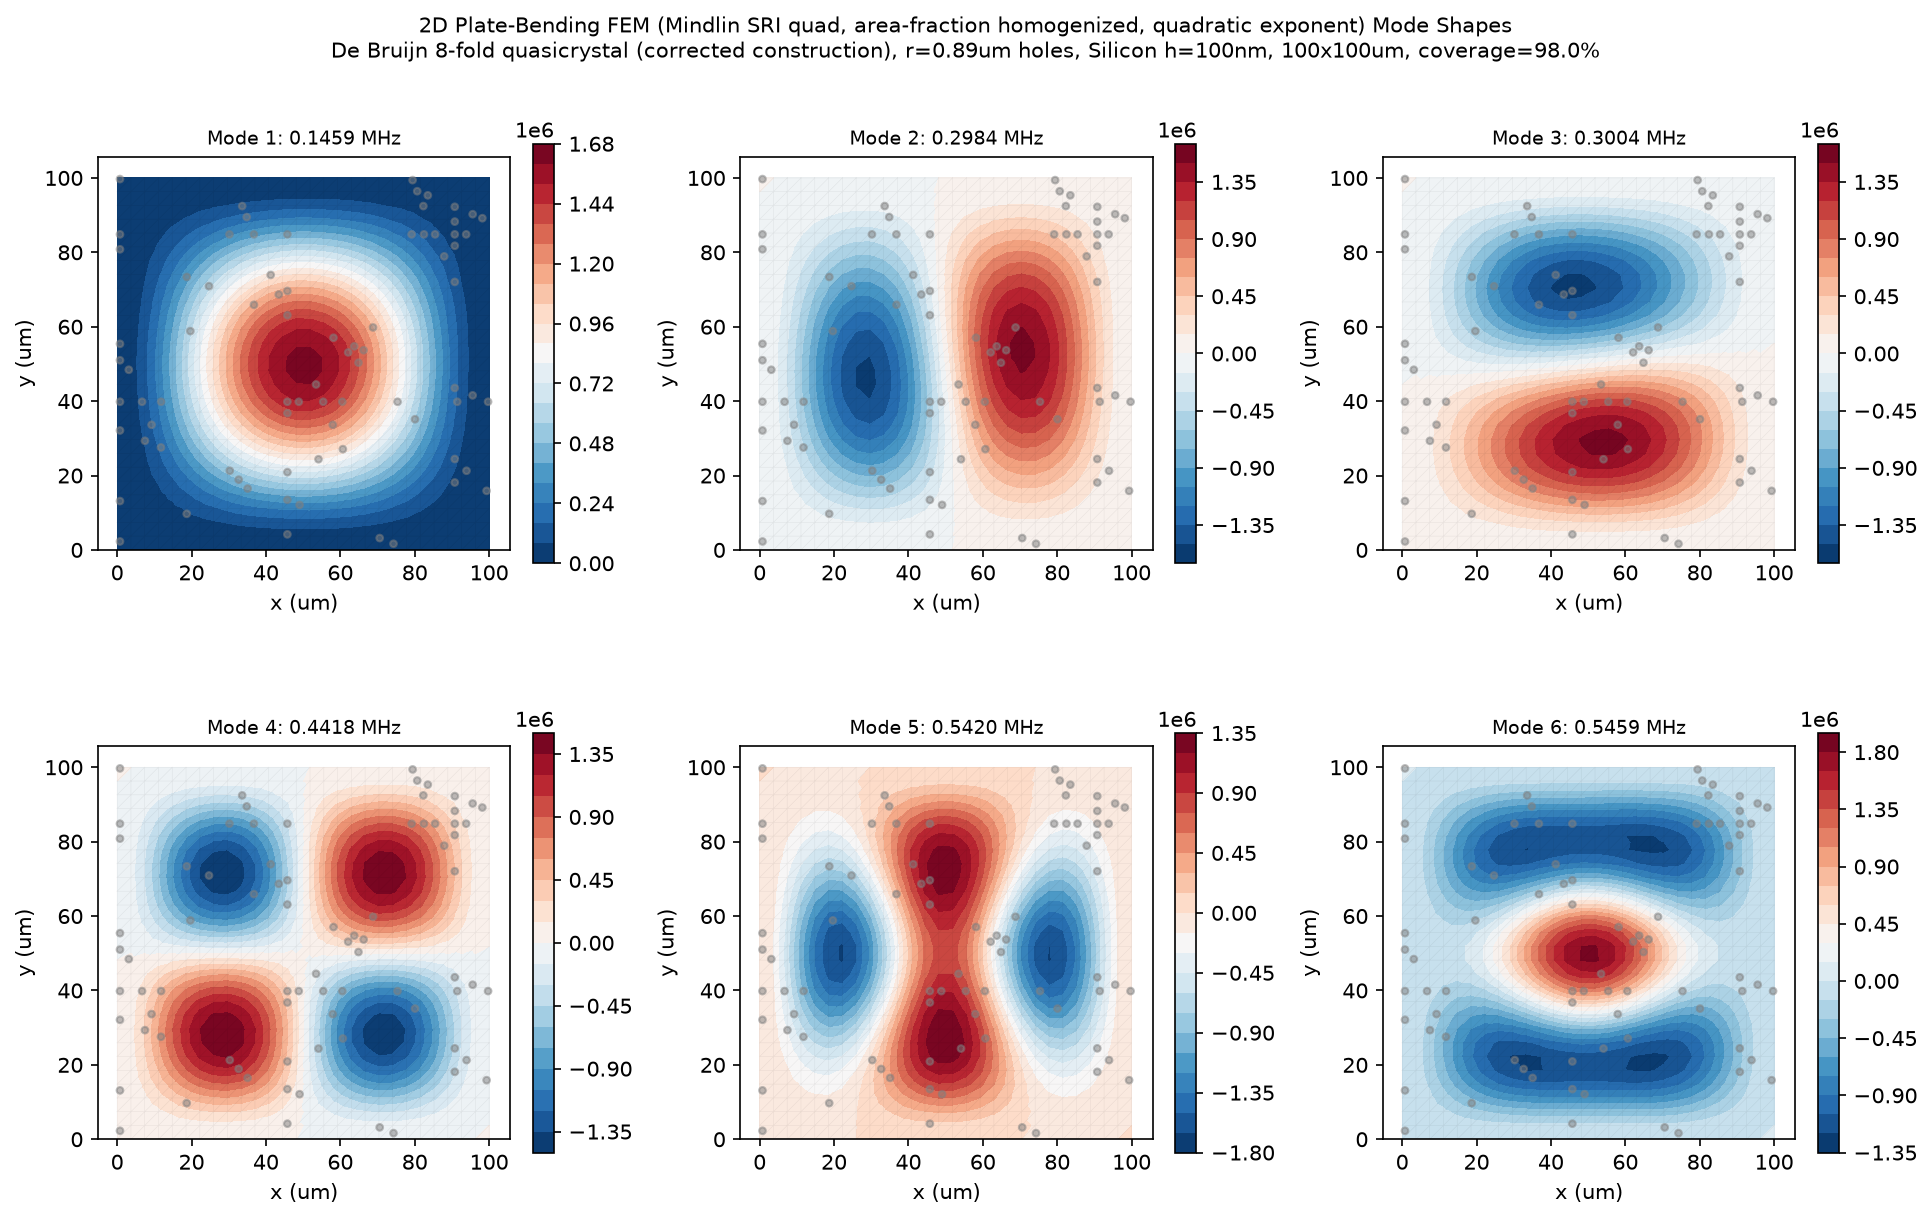
\includegraphics[width=0.85\textwidth]{figure_mode_shapes.png}
\caption{First six bending mode shapes, $n=8$ quasicrystal pattern, $\sim$98\% coverage.}
\label{fig:modeshapes}
\end{figure}

\subsection{Relationship to the earlier (binary-removal) phase of this study}
\label{sec:earlier-phase}

An earlier phase of this study, using the now-superseded binary-removal hole representation (Section~\ref{sec:methods-element}), reported no detectable symmetry effect at 98\% coverage (spread 0.14--0.31\%, within a 0.32--0.82\% noise floor), but could not evaluate 90\% or 80\% coverage at all due to non-converging mesh fragmentation. Two subsequent corrections --- the stiffness-exponent resolution (Section~\ref{sec:exponent}) and the de Bruijn construction bug fix (Section~\ref{sec:methods-element}) --- each revised the 98\%-coverage spread before settling on the value reported in Section~\ref{sec:symmetry-results} (0.15\%, still not detectable above its noise floor --- broadly, though not exactly, consistent with the original binary-removal-era result at this one coverage level, since the methods and numbers differ). The substantive correction from the earlier phase is not at 98\% coverage but at 90\% and 80\%, which binary removal could not evaluate at all, and which the corrected method now shows as real, detectable, growing effects.

\section{Discussion}

\subsection{Both coverage and symmetry order affect fundamental frequency; coverage's effect is larger}

Hole coverage is the dominant design variable across the full range tested (80--99.8\%). Rotational symmetry order has a real, independently detectable effect once coverage is properly controlled --- smaller than coverage's effect, and itself growing smoothly and monotonically as coverage decreases across all five coverage levels now tested (not statistically detectable at 98\%, real and growing from 94\% through 80\% --- Section~\ref{sec:symmetry-results}) --- rather than no effect at all, as an earlier (methodologically flawed) phase of this study had concluded. The direction of the effect is consistent across every coverage level where it is detectable (lower symmetry order associated with lower frequency at matched coverage), though five coverage points is still not enough to fit a specific functional form (e.g., linear vs.\ power-law in coverage loss) with confidence, and we have not tested symmetry orders beyond the four ($n=3, 6, 8, 12$) used throughout this study.

\subsection{A methodological correction, and what it cost and revealed}
\label{sec:limitations-discussion}

This study's most significant single finding may be methodological rather than physical. Three independent issues were found and corrected over the course of this work --- a non-converging binary-removal hole representation (Section~\ref{sec:methods-element}), an unresolved stiffness-penalization exponent (Section~\ref{sec:exponent}), and a de Bruijn point-generation bug that silently produced a too-sparse quasicrystal pattern (Section~\ref{sec:methods-element}) --- and all three share a common pattern: each produced internally consistent, individually-plausible results that passed informal scrutiny, and was caught only by checking more carefully than the working hypothesis or default modeling choice seemed to demand. The 90\%-coverage fragmentation check that mistakenly verified against the wrong hole radii, and the de Bruijn bug that was only caught while trying to write a precise, checkable description of the algorithm rather than trusting that the code matched its docstring, are both instances of the same lesson: a result consistent with what we already believed received less scrutiny than a contradicting one would have. We regard the corrected methodology and the qualitatively cleaner finding it ultimately produced --- no detectable symmetry effect at near-dense coverage, a real and growing effect as coverage decreases --- as more valuable than any of the original, individually-plausible-but-wrong intermediate results, or a paper that simply narrowed its claims around unresolved uncertainty without pursuing a resolution.

\subsection{Relationship to prior photonic and phononic-crystal literature, and a direct test of bandgap width}

In locally resonant phononic crystals, bandgap frequency has been reported to depend primarily on the resonance frequency of scattering units, with comparatively less dependence on periodicity/symmetry --- broadly consistent with coverage being the dominant variable found here, via a different physical mechanism (local resonance vs.\ plain structural bending-stiffness reduction). In 2D photonic quasicrystals, symmetry order produces a substantial, well-established effect on complete bandgap \textit{width} (16.5\% for an optimized 5-fold structure vs.\ 13.5\% for an optimized 8-fold structure \cite{florescu2009}) --- a different quantity from the fundamental-mode frequency tested in Section~\ref{sec:results}, since bandgap width measures the size of a forbidden frequency range between bands, not the value of any single mode.

We tested this directly. Using freshly coverage-matched (80\% target, $\pm$0.4\%, achieved cleanly for all four symmetry orders with the corrected de Bruijn geometry --- Section~\ref{sec:methods-element}) configurations and the quadratic stiffness exponent (Section~\ref{sec:exponent}), we computed the first 15 eigenfrequencies (rather than just the lowest) and identified the gap between the fundamental mode and the next band (gap 0--1) as a consistently-present, comparable feature across all four symmetry orders --- an initial attempt using the single largest gap among the first 15 modes was found to pick out a \textit{different} pair of modes for $n=6$ than for the other three symmetry orders, and was discarded as an unreliable metric for this reason. An earlier version of this test used the linear exponent, predating the exponent resolution in Section~\ref{sec:exponent}, and is superseded by the result below; a subsequent version used the corrected exponent but the pre-fix (buggy) de Bruijn geometry, and is also superseded.

With three seeds per symmetry order, gap 0--1's width (as a fraction of its midpoint frequency) was: 51.90\% ($n=3$, std$=19.14\%$, mean of seeds dominated by one outlier seed --- see below), 66.90\% ($n=6$, std$=1.35\%$), 68.15\% ($n=8$, std$=1.06\%$), and 69.37\% ($n=12$, std$=0.14\%$). \textbf{For $n=6$, 8, and 12 --- the three symmetry orders with low, well-behaved seed-to-seed noise --- this is a real, monotonically increasing trend} (spread 3.63\% across these three, against noise of 0.14--1.35\%, a clearly detectable signal). $n=3$'s mean is dragged down by a single outlier seed (24.85\% gap width, vs.\ 64.48\% and 66.38\% for its other two seeds --- those two alone are well within the $n=6$--$n=12$ range and consistent with the trend). We investigated this outlier directly: it is not a numerical artifact (no spurious or negative eigenvalues; the full mode spectrum is smooth and physically reasonable) but reflects a genuine geometric idiosyncrasy of that specific seed's hole arrangement, which produces three nearly-degenerate modes (within 0.2\% of each other) immediately above the fundamental, compressing the 0--1 gap for that particular configuration. This is plausible given $n=3$'s still-comparatively-low candidate-point count (12, vs.\ 39--140 for the other orders --- see Section~\ref{sec:methods-element}) even after the de Bruijn construction bug fix, and we report it rather than excluding it, since unlike the earlier (pre-correction) outlier discussed in Section~\ref{sec:limitations}, we have identified and can describe its specific cause.

\textbf{This reverses our earlier conclusion: rather than no detectable symmetry-order effect on bandgap width, the corrected (quadratic-exponent, corrected-geometry) result is a real, symmetry-order-dependent effect, qualitatively \textit{consistent with} --- not in contrast to --- the photonic quasicrystal literature}, in which higher symmetry order is similarly associated with larger optimized bandgaps \cite{florescu2009}. This does not establish the same underlying mechanism in both systems (mechanical bending-stiffness reduction vs.\ photonic Bragg-type scattering are physically distinct), the trend is most reliably established at $n=6$--$n=12$ ($n=3$'s high single-seed noise leaves its place in the trend suggestive rather than conclusively resolved), and the comparison remains based on a single gap (0--1) and coverage level ($\sim$80\%), so it should not be over-generalized to other gaps or coverage levels without further testing --- but the qualitative direction of the finding itself has changed, not merely its magnitude.

\subsection{Practical implication}

Hole coverage remains the primary, most easily controlled tuning variable for fundamental frequency. Rotational symmetry order is not negligible: its effect is not statistically detectable above our mesh-convergence noise floor at near-dense ($\sim$98\%) coverage, but a real, clearly detectable effect by 80--90\% coverage, of an order of magnitude approaching coverage's own effect. We would caution designers against assuming symmetry order is a free design parameter at any coverage level (as our initial, since-corrected analysis suggested); at near-dense coverage this caution may be less urgent in practice (we found no statistically detectable effect there, though this is a measurement-resolution statement, not a claim that no real effect exists), but symmetry order should not be assumed away in designs targeting more substantially perforated structures ($\sim$80--90\% coverage).

Designers should also weigh this against fabrication reality. Using the coverage-sensitivity slope measured directly in Section~\ref{sec:results} ($\sim$5.2\% frequency change over a 22.2-percentage-point coverage range, i.e., $\sim$0.23\%/percentage-point), a representative $\pm$2-percentage-point coverage fabrication tolerance would by itself produce a frequency shift of roughly 0.47\% --- well under both symmetry-order spreads (38\% of the 90\%-coverage spread, 10\% of the 80\%-coverage spread). This is a reassuring, if approximate, finding: at this level of fabrication tolerance, the symmetry-order effect should remain distinguishable from ordinary coverage-control variation at both coverage levels where it is detectable, rather than being swamped by it. This estimate borrows the coverage-sensitivity slope from a different configuration ($n=8$, linear exponent, $n_x=22$) than the symmetry comparison itself (quadratic exponent, $n_x=28$, varying $n_{\text{fold}}$), so it should be treated as an order-of-magnitude check, not a precise prediction.

\section{Limitations}
\label{sec:limitations}

\begin{itemize}
\item This model primarily captures fundamental bending-mode frequency; a single bandgap-width measure (gap 0--1, at $\sim$80\% coverage) was also tested directly (Section~\ref{sec:methods-element}) and showed a real, monotonically increasing effect of symmetry order, most reliably established between $n=6$ and $n=12$ (low noise) and only suggestive at $n=3$ (one high-noise outlier seed with an identified, non-numerical cause), but this has not been generalized to other gaps or coverage levels. Mode density, quality factor, and force sensitivity --- also of primary interest in \cite{li2026} --- were not computed.
\item The finite-element model has not been cross-validated against a commercial solver (e.g., COMSOL, ANSYS) or fabricated/measured hardware.
\item The independent second-element cross-validation (Section~\ref{sec:crossval}) now uses the corrected, quadratic-exponent methodology and the corrected de Bruijn geometry, with all four symmetry orders included (the $n=3$ coverage-matching ceiling present under the earlier, buggy geometry construction is resolved), but used only 5 seeds and a single coverage level (80\%), for computational practicality.
\item The area-fraction homogenization is itself an approximation, not an exact representation of sub-element-scale hole geometry; a fully conformal (constrained Delaunay) mesh, respecting true hole boundaries exactly, was not implemented and would be a more rigorous (if substantially more complex) alternative. The stiffness-penalization exponent within this homogenization --- initially an unresolved free choice that changed the reported symmetry-spread magnitudes by a factor of 2--3 --- was subsequently resolved (Section~\ref{sec:exponent}) by checking which exponent better matches an exponent-independent, fine-mesh reference value; this is itself a coarse-mesh approximation check, not a substitute for a fully conformal mesh. The original check used a single configuration ($n=8$, 80\% coverage); a follow-up check at three additional configurations ($n=3$/12 at 80\%, $n=3$/8 at 90\%) confirmed quadratic remains the better choice in all cases, though its margin over linear is much smaller at $n=3$ (where both exponents show 10--24\% error from a fine-mesh reference, a real $n=3$-specific mesh-convergence issue) than at $n=8$/12 (0.2--11\% error). The $\phi$-floor regularization value ($10^{-3}$) was separately checked for sensitivity and found robust ($\leq0.39\%$ deviation across three orders of magnitude in the floor value).
\item Coverage-matching used a bisection search with a stated target tolerance ($\pm0.4\%$); exact bit-for-bit reproducibility of specific hole radii was not established.
\item \textbf{The de Bruijn point-generation construction (Section~\ref{sec:methods-element}) contained a real implementation bug for most of this study's duration, producing an artificially sparse point pattern (most consequentially at low symmetry order: $n=3$ had only $\sim$5 candidate points pre-fix, vs.\ 12 post-fix). It was found, fixed, and re-verified before any results in this manuscript were finalized --- see Section~\ref{sec:methods-element} for the technical detail and Section~\ref{sec:limitations-discussion} for the broader methodological pattern it represents.}
\item Five seeds were tested per symmetry order per coverage level for the quadratic-exponent results (Section~\ref{sec:symmetry-results}), each individually coverage-matched. No outlier seeds were excluded from any reported mean --- the $n=3$, 80\%-coverage outlier present under the earlier (pre-de-Bruijn-fix) geometry does not recur under the corrected one. A different, smaller-scale outlier was found in the bandgap-width analysis (Section~\ref{sec:symmetry-results}, one $n=3$ seed) with an identified, non-numerical cause described there. $n=3$'s elevated mesh-resolution uncertainty (Section~\ref{sec:exponent}, above) compounds with this seed-to-seed noise.
\item We tested two intermediate coverage levels (85\%, 94\%; Section~\ref{sec:symmetry-results}) confirming smooth, monotonic growth in the symmetry-order effect across all five coverage points now tested, but five points is still not enough to fit a specific functional form (e.g., linear vs.\ power-law in coverage loss) with confidence, and these intermediate points used only 3 seeds per symmetry order (vs.\ 5 for the original three levels), for computational practicality.
\item Transient (propagating-wave) localization behavior (``rainbow trapping'') was tested separately in a simplified in-plane model and a 1D reduced-order bending model, both using the now-superseded binary-removal-style geometry construction in the in-plane case; the in-plane case did not show robust rainbow trapping, and this has not been revisited with the corrected geometry methodology.
\end{itemize}

\section{Conclusion}

In a finite-element model of a clamped, quasicrystal-perforated silicon MEMS plate, hole coverage is the dominant determinant of fundamental bending-mode frequency (10.51\% change, 98\%$\to$80\% coverage), and rotational symmetry order has a real, smaller, coverage-dependent secondary effect: not statistically detectable at near-dense (98\%) coverage, and clearly detectable by 90\% and 80\% coverage, with smooth, monotonic growth confirmed across all five coverage levels tested (Section~\ref{sec:symmetry-results}). This finding is the product of three methodological corrections made over the course of this study --- a non-converging binary element-removal hole representation (Section~\ref{sec:methods-element}), an unresolved stiffness-penalization exponent (Section~\ref{sec:exponent}), and a de Bruijn point-generation construction bug (Section~\ref{sec:methods-element}) --- discussed as a single epistemic lesson in Section~\ref{sec:limitations-discussion}. A direct test of bandgap width, using the fully corrected methodology, found a real, monotonically increasing symmetry-order effect at $\sim$80\% coverage (Section~\ref{sec:symmetry-results}), most reliably established at the low-noise $n=6$--$n=12$ end, qualitatively \textit{consistent with} --- not in contrast to --- the photonic quasicrystal literature, reversing an earlier, pre-correction null finding on this measure. We present the corrected physical finding, the corrected bandgap-width result, and the methodological corrections that produced both as the central contributions of this study.

\section*{Acknowledgments}

AI assistance disclosure: the finite-element code, the numerical experiments, and the successive rounds of self- and AI-assisted review documented in this study were developed with the assistance of Claude (Anthropic), used as a coding and analysis tool under the author's direction. This assistance includes the discovery and correction of all three methodological flaws described in the paper --- the binary-removal hole representation (Section~\ref{sec:methods-element}), the unresolved stiffness-penalization exponent (Section~\ref{sec:exponent}), and the de Bruijn point-generation bug (Section~\ref{sec:methods-element}) --- and the implementation of the independent cross-validation element (Section~\ref{sec:crossval}). The Abstract and the ``Summary of findings'' paragraph opening Section~\ref{sec:results} reflect the author's own understanding in the author's own words: the author was walked through each underlying concept (including the finite-element machinery, the homogenization, the exponent-calibration argument, and the methodological lesson) via a guided, Socratic process and asked to explain each back, and these passages were composed from those explanations rather than copied from AI-generated text. The remaining sections (detailed Methods, Results tables, Discussion, Limitations, Conclusion) were drafted with substantial AI assistance; the author has since worked through their technical content concept-by-concept via the same Socratic process, but the prose of those sections has not been independently rewritten by the author. All modeling decisions, interpretation of results, and the content of this manuscript are the responsibility of the author.

\begin{thebibliography}{9}

\bibitem{li2026}
K.~Li, H.~Cho, R.~Norte, D.~Shin, ``Quasicrystal Architected Nanomechanical Resonators via Data-Driven Design,'' \textit{arXiv:2604.07379} (2026).

\bibitem{florescu2009}
M.~Florescu, S.~Torquato, P.~J.~Steinhardt, ``Complete band gaps in two-dimensional photonic quasicrystals,'' \textit{Physical Review B} \textbf{80}, 155112 (2009); \textit{arXiv:1007.3555}.

\bibitem{leissa1969}
A.~W.~Leissa, \textit{Vibration of Plates}, NASA SP-160 (1969).

\bibitem{hughes1978}
T.~J.~R.~Hughes, M.~Cohen, M.~Haroun, ``Reduced and selective integration techniques in the finite element analysis of plates,'' \textit{Nuclear Engineering and Design} \textbf{46}(1), 203--222 (1978).

\bibitem{hughes1981}
T.~J.~R.~Hughes, T.~E.~Tezduyar, ``Finite elements based upon Mindlin plate theory with particular reference to the four-node bilinear isoparametric element,'' \textit{Journal of Applied Mechanics} \textbf{48}(3), 587--596 (1981).

\end{thebibliography}

\end{document}
